% ______________________________________________________________________________
%
%   2DV513 Database Theory -- Assignment 1
%
%   Author:  Jonas Sjöberg
%            Linnaeus University
%            js224eh@student.lnu.se
%            github.com/jonasjberg
%            www.jonasjberg.com
%
%  License:  Creative Commons Attribution 4.0 International (CC BY 4.0)
%            <http://creativecommons.org/licenses/by/4.0/legalcode>
%            See LICENSE.md for additional licensing information.
% ______________________________________________________________________________


\section{Task 4 --- Classroom Scheduling}
Based on an exercise from \emph{Database System Concepts, 5th Edition}
\cite{2dv513:dsc}, section 6.6.

\subsection{Problem Description}
The problem description \cite{2dv513:assignment1-instructions} is stated as
follows:

\begin{quote}
  Consider a university database for the scheduling of classrooms for the final
  exams.

  This database could be modeled as a single entity set \emph{exam} with
  attributes
  \emph{course\_name}, \emph{section\_number}, \emph{room\_number},
  and \emph{time}.

  Alternatively, one or more additional entity sets could be defined, along
  with relationship sets to replace some of the attributes of the \emph{exam}
  entity set, as:

  \begin{enumerate}
    \item
      \emph{course} with attributes \emph{name}, \emph{department},
      and \emph{c\_number}.

    \item
      \emph{section} with attributes \emph{s\_number} and \emph{enrollment},
      and dependent as a weak entity set on \emph{course}.

    \item
      \emph{room} with attributes r_number}, capacity, and building.
  \end{enumerate}

  Show an E/R diagram illustrating the use of all three additional entity sets
  listed.

  Explain what application characteristics would influence a decision to
  include or not include each of the additional entity sets.

  \emph{Note:} A section is a part of course. How sections are used varies from
  university to university, but they could for example be used to separate
  multiple versions of the course (imaging that a course has so many students
  that there has to be parallel lectures) or if a course is given multiple
  times per year.
\end{quote}


% \subsection{Solutions}
% See Figure~\ref{fig:task4}.
% 
% 
% \begin{figure}[htbp]
%   \centering
%   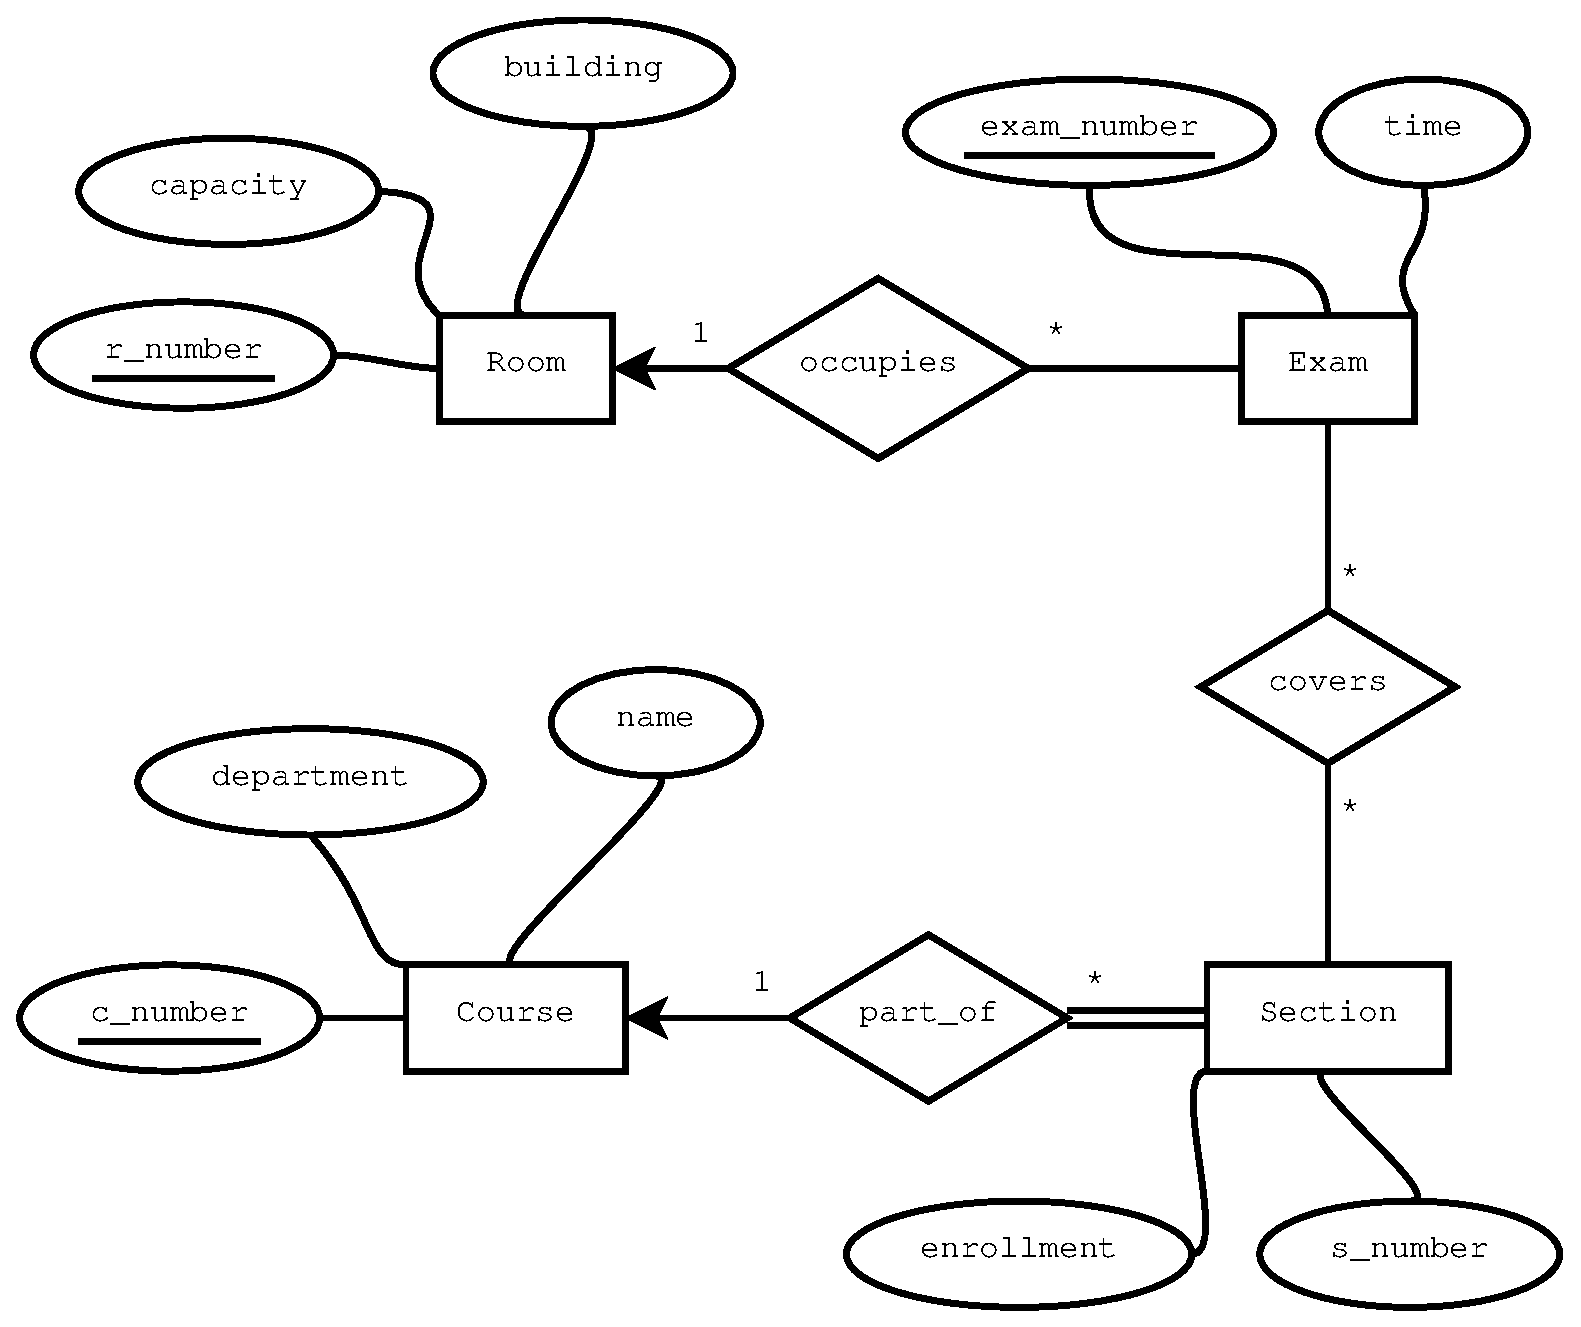
\includegraphics[width=\linewidth]{include/task4.eps}
%     \caption{Entity-relationship Diagram for Task 4}
%   \label{fig:task3}
% \end{figure}
